\chapter{Il teorema di Cauchy-Kowalevski} \label{invariant}

Adesso che abbiamo sviluppato tutti gli strumenti necessari, ipotizziamo di avere un problema di Cauchy qualsiasi. Come abbiamo mostrato nel paragrafo \ref{pb}, esso può essere riscritto nella forma:
$$
\begin{cases}
F(x,t, D^\alpha_x D^j_t u)=0 & |\alpha | +j \leq k\\
D^j_t u (x,0)= \phi_j(x) & \text{per }j<k 
\end{cases}
$$
Di conseguenza ci occuperemo solo di quest'ultimo caso, in cui le condizioni vengono assegnate su $\Gamma_0=\{ t=0 \}$.

L'assunzione fondamentale di questo capitolo è che i dati ($F$ e $\phi_j$) siano analitici in un intorno dell'origine, proprietà che utilizzeremo per mostrare l'esistenza di un'unica \textbf{soluzione analitica}, sempre in intorno dell'origine.

Per garantire l'esistenza, però, siamo costretti a fare qualche ipotesi sulla struttura dell'equazione. 
Considerando quanto è stato detto nel capitolo precedente, sopratutto per quanto riguarda il teorema \ref{teoescar}, l'intuito suggerisce che potrebbe essere una buona idea considerare che la superficie $\Gamma_0$ sia non caratteristica. 
Quindi, come seconda assunzione scegliamo la \textbf{non-caratteristicità} della superficie. Tale proprietà ci permette di riscrivere nuovamente l'equazione in un'altra forma, ancora più semplice, ovvero:
\begin{equation}\label{pbnorm}
\begin{cases}
D_{t}^k u = G(x,t, D^\alpha_x D^j_t u) & |\alpha |+ j \leq k, \, j<k \\
D_t^ju = \phi_j & \text{ su } \Gamma_0, \, j<k
\end{cases} \\
\end{equation}
Questa idea ci permetterà di dimostrare il TCK.
\begin{namedtheorem}[Teorema di Cauchy-Kowalevski]
\hpth{
\text{Problema \eqref{pbnorm}}\\
G, \, \phi_j \text{ analitici in intorno dell'origine}
}
{\exists ! \; u \text{ soluzione analitica in intorno dell'origine}}
\end{namedtheorem}


Dopo aver mantenuto uno sguardo quanto più generale possibile, ci vogliamo occupare di capire come di mostrare il risultato che abbiamo in mente. L'approccio che seguiremo sarà ``al contrario'', ovvero generalizzando progressivamente i risultati. Infatti, partiremo dal caso meno generale, fino ad arrivare a quello di un'equazione in forma normale, seguendo di fatto l'ordine cronologico di scoperta.




\newpage
\section{EDO}

Per prima cosa affrontiamo un teorema molto simile al TCK, che tratta il caso di un sistema di EDO in forma normale.
Cominciamo subito col riportare l'enunciato.

\begin{theorem}\label{teoedo}
\hpth{
A \subseteq \mathbb{C}, \, B\subseteq \mathbb{C}^n \text{ aperti }\\
\Omega \subseteq A \text{ aperto connesso}\\
f:A\times B\rightarrow\mathbb{C}^n \text{ olomorfa}\\
\text{Pb: }
\begin{cases}
y' = f(x,y) \quad \forall x \in \Omega \\
y(x_0)=y_0
\end{cases}\\
}
{
\text{localmente esiste un'unica soluzione olomorfa}
}
\end{theorem}

\begin{remark}
Non esclude la possibilità di trovare altre soluzioni non analitiche.
\end{remark}

Questo risultato fu la prima applicazione della teoria delle funzioni olomorfe in combinazione al metodo dei maggioranti, la quale, come già sappiamo, è stata proposta da Cauchy nella prima metà dell'Ottocento.
Non riportiamo la dimostrazione per esteso, perché utilizza un maggiorante diverso rispetto a quello che abbiamo introdotto nel paragrafo \ref{seriedipotenze} (ovvero quello che utilizzeremo per dimostrare il TCK). 
In ogni caso, può essere trovata in \cite{Delf} e la struttura del ragionamento è la stessa del teorema \ref{teoquasilin}.

Nonostante non affrontiamo la questione dell'esistenza nel dettaglio, è conveniente discutere a parole e in modo esaustivo il problema dell'\textbf{unicità} di soluzioni analitiche (o olomorfe). Una funzione analitica è univocamente determinata da tutte le sue derivate in un punto, le quali, in questo caso, sono note grazie all'analiticità della funzione $f$.
Chiudiamo completamente il discorso affrontando anche la situazione di una EDP: anche qui, assumendo i dati analitici, è possibile conoscere tutte le derivate parziali della funzione, grazie all'ipotesi di non-caratteristicità della superficie su cui vengono assegnate le condizioni.

Poiché questo risultato è stato dimostrato costruendo un maggiorante per la soluzione $y$, è possibile ottenere una stima del suo raggio di convergenza sfruttando il teorema \ref{teomagg}.

\begin{theorem}
\hpthml{
\text{Ipotesi del teorema \ref{teoedo}}\\
\exists \, \overline{B_a(x_0)}\subseteq A,\,\overline{B_b(y_0)} \subseteq B\\
M=\max_{B_a(x_0),\, B_b(y_0)}|f|
}{
\text{La soluzione ha raggio almeno } \widetilde{r}= a\left[ 1-\exp\left( -\frac{b}{aM(n+1)}\right) \right] 
}
\end{theorem}

\begin{remark}
E' interessante osservare cosa accade quando $B=\mathbb{C}^n$.
\end{remark}




\newpage
\section{EDP quasi-lineari}

Ora è il momento di trattare la chiave di volta di tutto il ragionamento sulle EDP, ovvero il teorema che mostra l'esistenza, e quindi anche l'unicità, di una soluzione analitica a un sistema quasi-lineare di EDP in forma normale.

\begin{theorem}\label{teoquasilin}
\hpth{
A_i , \, B\text{ analitici in un intorno dell'origine }\\
\text{Pb: }
\begin{cases}
D_t \, y = \sum\limits_{i=1}^{n-1} A_i(x,y)D_{x_i}y+B(x,y) \; \\
y=0 \quad \text{ su } \Gamma_0
\end{cases}
\\
}{
\exists ! \; y(x,t): \mathbb{R}^n \rightarrow \mathbb{R}^m
\text{ sol. analitica in intorno dell'origine}
}
\end{theorem}

\begin{remark}
Questo teorema può essere tranquillamente modificato sostituendo l'analiticità con l'\textbf{olomorfia}, in modo da ottenere un enunciato simile al caso delle EDO, poiché l'estensione è immediato, in quanto nella dimostrazione non si fa alcuna particolare assunzione che distingue il caso reale da quello complesso.
\end{remark}



\begin{proof}
\begin{enumerate}
\item ipotizziamo $y_h = \sum c^h_{\alpha j} x^\alpha t^j$
\item inserendo le serie di $y,\, A_i,\, B$ si ottiene che: 
$$ c^h_{\alpha j} = Q^h_{\alpha j}(\text{coeff. delle serie di }A_i, \, B)$$
$Q$ polinomio a coefficienti non negativi
\item $\widetilde{A}_i \gg A_i, \, \widetilde{B} \gg B \implies \widetilde{y} \gg y$ grazie a $Q$
\item si scelgono $\widetilde{A}_i, \, \widetilde{B}$ in modo da poter calcolare esplicitamente $\widetilde{y}$ analitica con il metodo delle caratteristiche

Sistema maggiorante

Come sappiamo già fare, maggioriamo le serie con 
$$\mathcal{M}_{Cr}(x,y) \gg A_i(x,y),\, B(x,y)$$
e risolviamo il problema\footnote{con $h=1,\ldots, m$}:
\begin{equation*}
\begin{cases}
D_t \, \widetilde{y}_h = \mathcal{M}_{Cr} (x,y) \left[\sum\limits_{i,\, j} D_{x_j}\widetilde{y}_i+1 \right] \\
\widetilde{y_h}=0 \quad \text{ su } \Gamma_0
\end{cases}
\end{equation*}



Soluzione maggiorante

Il sistema precedente ha come soluzione:
\begin{equation}\label{maggiorante}
\widetilde{y}_h(x,t)=u(x_1+\cdots +x_n,\,t) \quad \forall h
\end{equation}
con
\begin{equation}\label{sol}
u(s,t)=\frac{r-s-\sqrt{(r-s)^2-2tCrmn}}{mn}
\end{equation}
che è chiaramente analitica in intorno dell'origine. Nota bene: $\widetilde{y}$ è effettivamente maggiorante se $|(x,\widetilde{y}(x,t))|< r$ (in modo che $\mathcal{M}_{Cr}$ sia effettivamente una serie di potenze), vedi proposizione ...
\end{enumerate}
\end{proof}

\noindent\rule[0.5ex]{\linewidth}{0.2pt}

Come prima, se sfruttiamo il teorema, possiamo stimare il raggio di convergenza, studiando il raggio del maggiorante in \eqref{maggiorante}. 

\begin{theorem}
La soluzione del teorema \ref{teoquasilin} converge con raggio almeno
$$\widetilde{r} = \dfrac{1}{n-1}\, \dfrac{r}{8Cmn} \text{ con } C \geq \frac{1}{2}$$
\end{theorem}
\begin{remark}
$n \geq 2$ affinché il sistema si realmente alle derivate parziali. 
\end{remark}
\begin{remark}
E' interessante soffermarsi sull'andamento rispetto a $r$ (trade-off $Cr$), sapendo che:
\begin{align*}
r <& \min \{ \textit{raggi di conv. dei coefficienti } a^i_{ml}, \, b_m\} \\
C \geq & \max \begin{Bmatrix}
\max\limits_{i,m,l,\alpha } \left| (a^i_{ml})_\alpha \, r^{|\alpha |}\right|\\
\max\limits_{m,\alpha} \left|(b_m)_\alpha \, r^{|\alpha |}\right|
\end{Bmatrix}
\end{align*}
\end{remark}


\begin{proof}
Fissiamo $r$ e $C$ come sopra, inoltre ipotizziamo che $C\geq 1/2$ (possiamo farlo senza alcun problema). 
La funzione in \eqref{sol} è analitica in un intorno dell'origine, in particolare nell'insieme 
$$A = \left\{ (s,t) \in \mathbb{R}^2 : t<\frac{(r-s)^2}{2Crmn} \right\} .$$
\begin{center}
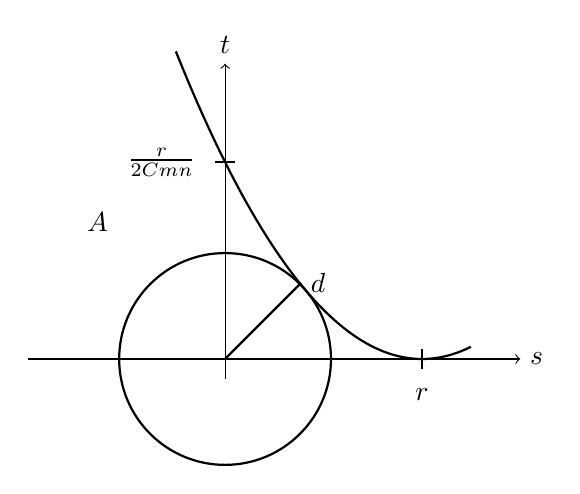
\begin{tikzpicture}[scale=2.5]
    % Disegna il cerchio con centro in (0,0) e raggio 0.538
    \draw[thick,black] (0,0) circle[radius=0.538];
    
    % Disegna la parabola y = (1-x)^2
    \draw[thick,black,domain=-0.25:1.25,samples=100] 
        plot ({\x}, {(1-\x)^2});
    
    \node[black,anchor=south west] at (-0.75, 0.60) {$A$};
    
    % Disegna gli assi
    \draw[->] (-1,0) -- (1.5,0) node[right] {$s$};
    \draw[->] (0,-0.1) -- (0,1.5) node[above] {$t$};
    
    % Disegna il segmento da (0,0) a (sqrt{0.538/2}, sqrt{0.538/2})
    \draw[thick,black] (0,0) -- (sqrt{0.538/1.9},sqrt{0.538/1.9});
    \node at (sqrt{0.538/1.9},sqrt{0.538/1.9}) [right] {$d$};
    
    % Disegna le tacchette richieste
    \draw[thick] (1, 0.05) -- (1, -0.05); % Tacchetta in (1, 0)
    \node at (1, -0.1) [below] {$r$};    % Etichetta per (1, 0)
    
    \draw[thick] (-0.05, 1) -- (0.05, 1); % Tacchetta in (0, 1)
    \node at (-0.1, 1) [left] {$\frac{r}{2Cmn}$}; % Etichetta per (0, 1)
    
\end{tikzpicture}
\end{center}

Ovvero è sviluppabile in serie di potenze in $B_l(0)$ con $0<l<d=\text{dist}(0, \partial A)$.
Scegliendo $l = \widetilde{r}$ si può dimostrare che, per $C>1/8$, si ha effettivamente che $l<d$. Per fare questo è sufficiente mostrare questa proprietà per $l=r/(8Cmn)$. L'obiettivo sarebbe, quindi, verificare che $$\sqrt{l^2-s^2} < \frac{(r-s)^2}{2Crmn}$$ per ogni $|s|<l$, ma ciò è implicato da 
$$l < \frac{(r-l)^2}{2Crmn}\; ,$$ disuguaglianza che risulta vera se e solo se $C > 1/(4mn) \leq 1/8$.
\end{proof}

\noindent\rule[0.5ex]{\linewidth}{0.2pt}

Un lettore attento sicuramente si chiederà la ragione dietro alla scelta di un costante $C\geq 1/2$ e del fattore $1/(n-1)$ per la definizione $\widetilde{r}$. Ebbene, questo problema emerge da un aspetto lasciato aperto nella dimostrazione del teorema \ref{teoquasilin}, ovvero il fatto che in realtà la soluzione $\widetilde{y}$ è veramente maggiorante solo se $|(x,\widetilde{y}(x,t))|< r$. Tale proprietà è proprio garantita in una palla di raggio $\widetilde{r}$. Vediamolo con una proposizione che, oltre a chiarire, completa il quadro logico delle dimostrazioni.
\begin{namedtheorem}[Proposizione]
La maggiorazione di $\widetilde{y}$ vale in $B_{\widetilde{r}}(0)$, ovvero
$$|(x,t)|<\widetilde{r} \implies |(x,\widetilde{y}(x,t))|=x_1^2 + \ldots + x_{n-1}^2 + m \, u^2(x_1 + \ldots + x_{n-1},t) < r^2$$
\end{namedtheorem}
\begin{proof}

\end{proof}

\newpage
\section{EDP in forma normale}
Ora ci occupiamo di sfruttare i risultati del paragrafo precedente per generalizzare quel risultato al caso di un'equazione in forma normale. Per fare ciò è sufficiente enunciare e dimostrare il seguente teorema.
\begin{theorem}\label{teonorm}
I due problemi seguenti sono equivalenti
\begin{align*}
\text{non lineare : }&
\begin{cases}
D_{t}^k u = G(x,t, D^\alpha_x D^j_t u) & |\alpha |+ j \leq k, \, j<k \\
D_t^ju = \phi_j & \text{ su } \Gamma_0, \, j<k
\end{cases} \\
\text{quasi-lineare : }&
\begin{cases}
D_t \, y = \sum\limits_{i=1}^{n-1} A_i(x,y)D_{x_i}y+B(x,y) \; \\
y=0 \quad \text{ su } \Gamma_0
\end{cases}
\end{align*}
\end{theorem}

\begin{proof}
si divide il ragionamento in tre passi:
\begin{enumerate}
\item si costruisce il sistema in modo tale che $y_{\alpha j}= D^\alpha_x D^j_t u$. \\
Quindi, le matrici $A_i$ e $B$ saranno quindi ricavabili dalle espressioni\footnote{$l(\alpha)=\min\{ l:\alpha_l\neq 0 \} $}
\begin{align*}
D_t y_{\alpha j} =& y_{\alpha (j+1)} & |\alpha| + j < k \\
D_t y_{\alpha j} =& D_{x_l} y_{(\alpha-e_l)(j+1)} & |\alpha| + j = k, \; j < k\\
D_t y_{0k} =& D_tG + \sum_{|\alpha|+j < k} D_{y_{\alpha j}}G y_{\alpha (j+1)} \\
& + \sum_{|\alpha|+j = k, \; j < k} D_{y_{\alpha j}} G D_{x_l} y_{(\alpha-e_l)(j+1)}
\end{align*}
e i dati di Cauchy saranno
\begin{align*}
y_{\alpha j}(x, 0) = & D_x^{\alpha} \phi_j(x) & j < k\\
y_{0k}(x, 0) = & G\left( x, 0, D_x^{\alpha} \phi_j(x) \right) & \lvert \alpha \rvert + j \leq k, \; j < k
\end{align*}
\item si rimuovono le condizioni $\phi$, ridefinendo $y(x,t)\leftarrow y(x,t)-\phi (x)$;
\item si rimuove la dipendenza da $t$, aggiungendo la variabile $y^0=t$, insieme all'equazione $D_t y^0=1$ e al dato $y^0(x,0)=0$.
\end{enumerate}
Concludiamo dicendo che ovviamente se $u$ è soluzione del problema in forma normale, le $y_{\alpha j}$ saranno soluzione del problema appena costruito. Ma per dimostrare che la $y_{(0,\ldots,0)}$ (soluzione di quest'ultimo) è anche soluzione del problema in forma normale sono necessari diversi conti che possono essere trovati per esteso in \cite[cap.1]{Folland}.
\end{proof}

\begin{remark}
Ci sono tre aspetti, che emergono anche dalla dimostrazione, su cui è il caso di soffermarsi brevemente a riflettere:
\begin{itemize}
\item mettendo insieme le considerazioni fatte all'inizio del capitolo e i teoremi \ref{teoquasilin} e \ref{teonorm}, segue in modo immediato il TCK;
\item continua a valere la stima del raggio di convergenza;
\item questo teorema di equivalenza si generalizza in modo immediato al caso di un sistema in forma normale.
\end{itemize}
\end{remark}








